% !TeX root = ../../main.tex
% ------------------------------------------------------------------
%  4.2.3 Servicios contratados en la plataforma de nube.
%
%  Aquí se resume por función; el listado servicio por servicio está en el
%  El detalle de servicios y cantidades se entrega en el T-11.
% ------------------------------------------------------------------

\section{Servicios contratados en la plataforma de nube}
\label{sec:servicios-nube}

La plataforma de nube es Amazon Web Services. Todos los servicios se contratan en cuentas del CLIENTE, organizadas bajo AWS Control Tower con una cuenta por ambiente, de modo que la propiedad de los datos y de la infraestructura es del CLIENTE desde el primer día. La selección sigue tres reglas:

\begin{itemize}
  \item Preferir el servicio administrado cuando existe, porque el área de TI del CLIENTE es de cuatro personas.
  \item Preferir servicios compatibles con estándares abiertos, para acotar el esfuerzo de salir de la plataforma.
  \item Contratar en la región secundaria solo lo que la recuperación ante desastres necesita.
\end{itemize}

\subsection{Servicios por función}

La Tabla~\ref{tab:servicios-nube} agrupa los servicios contratados por la función que cumplen en la arquitectura y los asocia a los componentes del catálogo que los usan. El listado servicio por servicio, con su justificación y su cantidad, se entrega en el Formulario T-11.

\begin{tablalafrox}{Servicios contratados en la plataforma de nube, por función}{tab:servicios-nube}%
  {F{0.21} Y F{0.19} F{0.17}}%
  {\cab{Función} & \cab{Servicios contratados} & \cab{Componentes} & \cab{Región}}
  Entrada pública & Route 53, CloudFront, AWS WAF, Shield Advanced, API Gateway pública & N-01 a N-03, N-12 & Global y sa-east-1 \\
  Acceso interno & Verified Access, API Gateway privada y endpoint execute-api & N-04, N-12 & sa-east-1 y us-east-1 \\
  Cómputo de aplicación & ECS Fargate, Application Load Balancer privado, Lambda autorizadora & N-04, A-05 & sa-east-1 y us-east-1 \\
  Datos operacionales & Aurora PostgreSQL, Database Migration Service, DynamoDB, ElastiCache & N-05, A-02, N-06, N-07 & sa-east-1 y us-east-1 \\
  Mensajería & SQS FIFO para la reconciliación y para las solicitudes al ERP y sus respuestas, SQS para los trabajos de Laravel y SNS, con equivalentes vacíos creados por infraestructura como código en us-east-1 & N-09, A-03 & sa-east-1 y us-east-1 \\
  Integración B2B & Network Load Balancer y OpenAS2 en Fargate & N-04 (M11) & sa-east-1 \\
  Internet de las cosas & IoT Core, IoT Greengrass & N-08, B-02, B-03 & sa-east-1 y borde \\
  Analítica & S3, Glue, Redshift Serverless, QuickSight embebido & N-10 & sa-east-1 \\
  Respaldo y recuperación & AWS Backup, S3 Object Lock, replicación de S3 entre regiones & N-11, D-05 & sa-east-1 y us-east-1 \\
  Red y conectividad & VPC, Transit Gateway, Site-to-Site VPN, NAT Gateway, VPC Endpoints & D-01 & sa-east-1 y us-east-1 \\
  Identidad, claves y secretos & KMS, Secrets Manager, Parameter Store, IAM Identity Center & A-05, N-12 & sa-east-1 y us-east-1 \\
  Detección y cumplimiento & Security Lake, GuardDuty, Security Hub, Inspector, Macie, CloudTrail, Config & N-12, F-03 & sa-east-1; CloudTrail, GuardDuty y Config también en us-east-1 \\
  Operación y gobierno & CloudWatch, Systems Manager, Control Tower, Organizations, Cost Explorer, Budgets & F-01, F-02, N-12 & sa-east-1 \\
  Construcción y registro de imágenes & CodeBuild y Elastic Container Registry con replicación de imágenes entre regiones & N-04, A-01 & sa-east-1 y us-east-1 \\
  Servicios de terceros en nube & Android Enterprise y Zebra DNA; consola del EDR & N-13, F-03 & Servicio gestionado \\
\end{tablalafrox}

{\footnotesize Fuente: elaboración propia.\par}

La tabla distingue los servicios de entrada, aplicación y datos. La aplicación corre en contenedores administrados; la única función Lambda autoriza las API REST. Los portales Angular se sirven desde S3 privado por CloudFront, mientras el frontend de consolas y el transporte AS2 mantienen dos tareas Fargate en dos zonas cada uno; el motor de rutas ejecuta una tarea por corrida. Las colas SQS de trabajos de Laravel están separadas de la cola FIFO de reconciliación; ElastiCache solo actúa como caché. El recorrido de acceso se precisa en la sección~\ref{sec:conexiones}.

\subsection{Región secundaria y residencia de los datos}

La región us-east-1 no es una segunda producción. Solo contiene recursos para la recuperación:

\begin{itemize}
  \item Datos: réplica de Aurora mediante Aurora Global Database y de las tablas de temperatura de DynamoDB mediante Global Tables.
  \item Respaldos: copia de los buckets de S3 salvo el de geolocalización y copias de AWS Backup.
  \item Aplicación: réplica reducida de ECS que escala a carga completa en menos de 30 minutos durante una conmutación.
\end{itemize}

La región primaria sa-east-1 está en São Paulo, Brasil, y la secundaria us-east-1 en Virginia del Norte, Estados Unidos; ambas suponen transferencia internacional de datos desde Chile. Los datos de geolocalización de personas quedan fuera de la región secundaria; la analítica se copia a ella en forma diferida, sin las posiciones de flota, porque conserva los registros de temperatura y de trazabilidad de lote que el caso exige retener cinco años (PUCV, 2026a, cap.~15, p.~26). La base de licitud, los resguardos de tratamiento y la garantía de continuidad ante las decisiones de residencia del CLIENTE se desarrollan en la sección~\ref{sec:e-especificaciones-del-sitio-secundario-y-}.

\subsection{Servicios que no se contratan}

Los registros de decisión descartan de forma expresa los siguientes servicios y productos, que no aparecen en la arquitectura:

\begin{itemize}
  \item No se instala Redis ni Laravel Horizon en los sitios, porque la continuidad local descansa en PostgreSQL y RabbitMQ, y un tercer motor por sitio agregaría operación sin beneficio.
  \item No se contrata un clúster de Kubernetes (EKS), porque el caso no exige desplegar ni escalar cada módulo por separado y el equipo de TI no operaría su plano de control.
  \item No se contrata Kafka administrado (MSK), porque RabbitMQ en cada sitio y SQS FIFO en la nube resuelven el orden y la durabilidad con menos operación.
  \item No se contratan servicios de trazas y métricas separados de CloudWatch, porque las Bases piden una sola plataforma de observabilidad para nube y on-premise.
  \item No se autoaloja un gestor de secretos, porque Secrets Manager rota las credenciales sin el desellado manual que exigiría uno propio.
\end{itemize}

\subsection{Modelo de contratación}

Los servicios se contratan por uso, con la capacidad base comprometida mediante Savings Plans y el peak de septiembre cubierto con capacidad efímera que se libera al terminar. Los ambientes de Desarrollo, QA y Preproducción se reducen o apagan fuera del horario de uso. La reversibilidad está asegurada por la elección de servicios: Aurora es compatible con PostgreSQL, los datos analíticos se guardan en formato Parquet, y Keycloak, Laravel, PostgreSQL y RabbitMQ son de código abierto, de modo que un traslado a otra plataforma conserva la aplicación y los datos y se concentra en sustituir los servicios administrados de AWS que la solución consume. Ese esfuerzo se acota en tres grupos: Aurora, ElastiCache, S3 y ECS Fargate se reemplazan por PostgreSQL, Redis, almacenamiento compatible con S3 y contenedores, solo con cambios de configuración; SQS, SNS, Secrets Manager y CloudWatch se reemplazan cambiando el adaptador que ya los aísla detrás de un puerto de la aplicación; e IoT Core con Greengrass, DynamoDB, Redshift con Glue y QuickSight, API Gateway con su autorizador y Verified Access no son portables y exigen rediseñar la ingesta de frío, la analítica y la entrada. Una salida cambia así la configuración de cuatro servicios y los adaptadores de otros cuatro, y rediseña cinco componentes (RT-03.07; PUCV, 2026b, cap. 3, p. 8). Los montos de estos servicios se declaran en la Oferta Económica y no en este documento.

\subsection{Topología de los servicios}

La Figura~\ref{fig:nube} ubica en la topología de AWS los servicios de la Tabla~\ref{tab:servicios-nube} y los recursos de la región secundaria: el borde global, la región primaria sa-east-1 con sus dos zonas de disponibilidad y la región de recuperación us-east-1. Los servicios de gobierno de cuentas de la tabla (Control Tower, Organizations, Cost Explorer y Budgets) se aplican sobre las cuentas y no ocupan un lugar en la topología, por lo que no se dibujan.

\begin{landscape}
\begin{figure}[p]
  \centering
  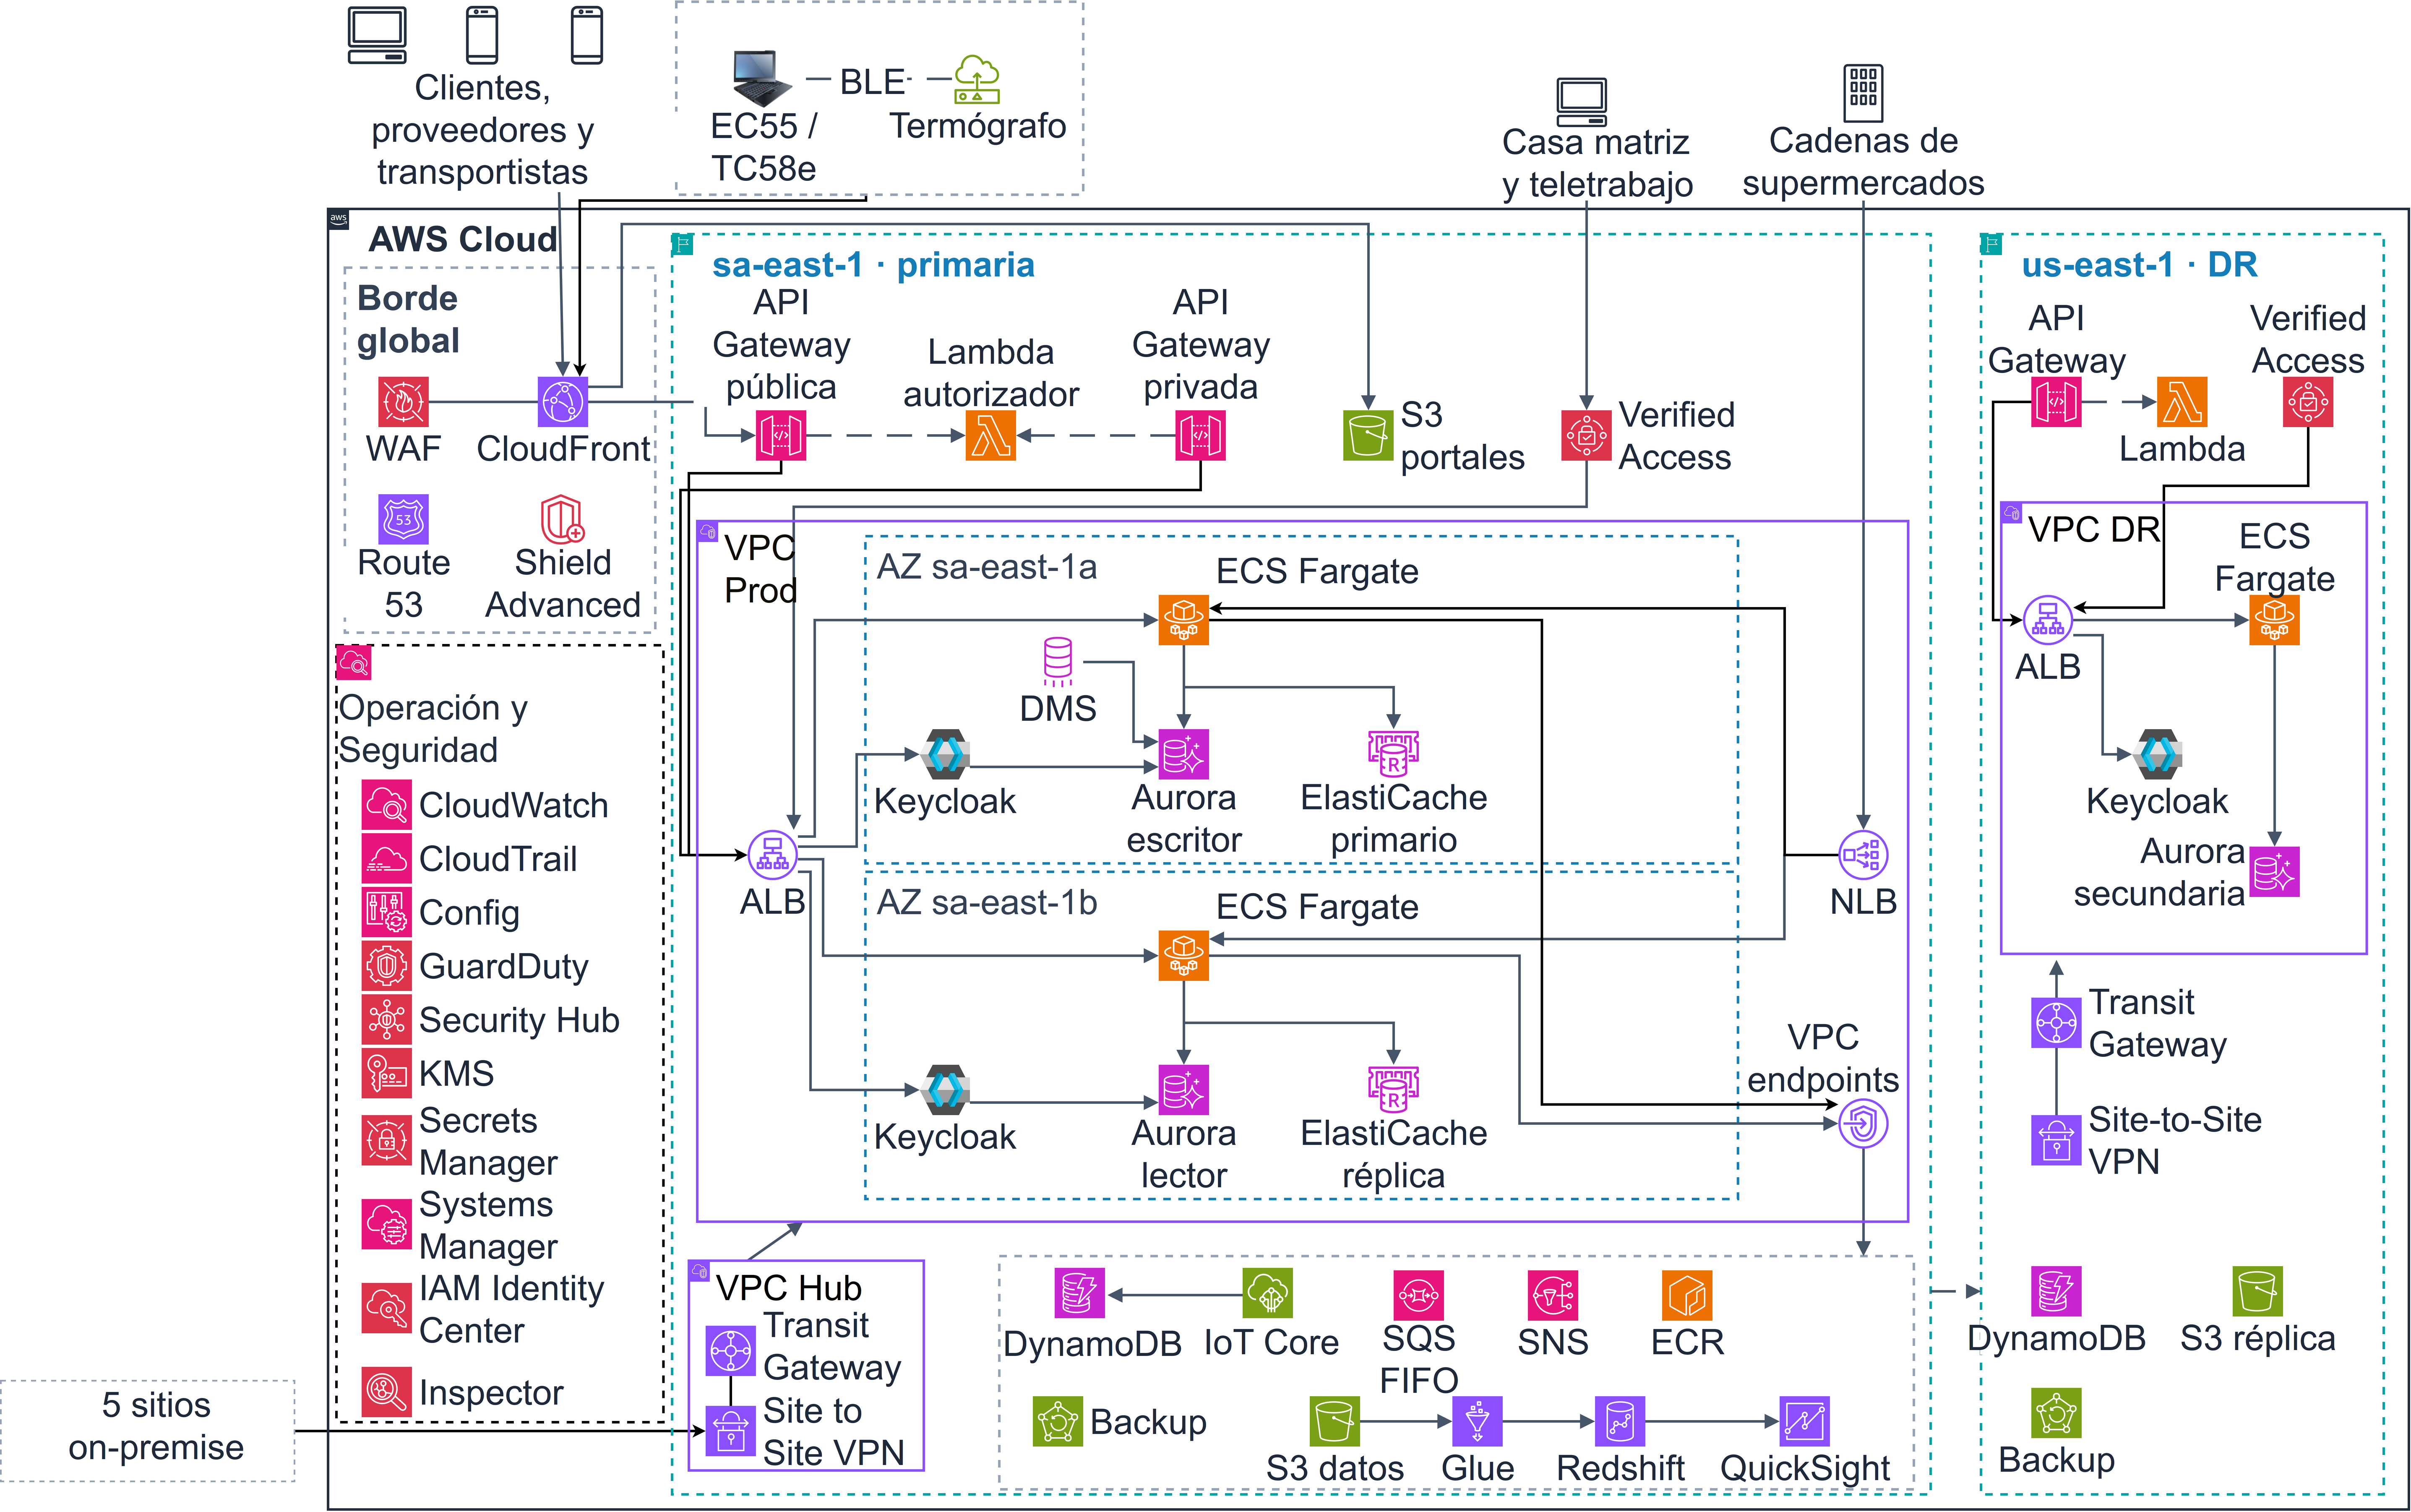
\includegraphics[width=\linewidth,height=0.9\textheight,keepaspectratio]{figuras/fisica/Arquitectura_Fisica_Nube.png}
  \caption{Topología de los servicios en AWS: región primaria sa-east-1 y región de recuperación us-east-1}
  \label{fig:nube}
  \fuentefigura
\end{figure}
\end{landscape}

La figura se recorre desde la entrada. En el borde global, Route 53 resuelve los nombres, y AWS WAF y Shield Advanced protegen a CloudFront, que sirve los portales desde S3 y reenvía las llamadas a la API Gateway pública. La Lambda autorizadora valida el token de las rutas protegidas de la API pública y de la API privada; los endpoints OIDC de autenticación pasan sin autorizador hacia Keycloak. La casa matriz y el teletrabajo entran por Verified Access al balanceador privado de aplicación, y las cadenas de supermercados llegan por el Network Load Balancer al transporte AS2.

Dentro de la VPC de producción, cada zona de disponibilidad tiene su propia copia de ECS Fargate, Keycloak y ElastiCache. Aurora PostgreSQL tiene el escritor en sa-east-1a y el lector promovible en sa-east-1b, y AWS DMS escribe en el escritor la réplica del PostgreSQL de Talca. Los VPC endpoints conectan Fargate con los servicios regionales sin salir a Internet. Esos servicios quedan fuera de las zonas porque AWS los opera en varias zonas de forma nativa: IoT Core escribe las lecturas de frío en DynamoDB, SQS FIFO recibe la reconciliación de los sitios, SNS difunde las alertas, ECR guarda las imágenes y AWS Backup custodia las copias; la analítica fluye de S3 a Glue, Redshift y QuickSight. El bloque de operación y seguridad (CloudWatch, CloudTrail, Config, GuardDuty, Security Hub, KMS, Secrets Manager, Systems Manager, IAM Identity Center e Inspector) es transversal a toda la región, y la VPC Hub recibe los túneles de los cinco sitios.

La región us-east-1 repite la cadena de entrada con capacidad reducida: API Gateway, la Lambda autorizadora, Verified Access y una VPC de recuperación con balanceador, Fargate, Keycloak y la réplica secundaria de Aurora, además de su propio Transit Gateway y su VPN para reconectar los sitios. La figura muestra así dos propiedades del diseño: ningún componente con estado depende de una sola zona de disponibilidad, y la recuperación regional no exige reconstruir la entrada, porque la réplica solo escala. Los tiempos de esa conmutación se fijan en el apartado~\ref{cap:4-3-data-center}.
